\documentclass[oneside]{book}
\usepackage[spanish]{babel}
\usepackage[utf8]{inputenc}
\usepackage[T1]{fontenc}
\usepackage{graphicx}
\usepackage{amsmath}
\usepackage{amsthm}
\usepackage[
  top=3cm,
  bottom=3cm,
  left=2cm,
  right=2cm,
  heightrounded,
]{geometry}
\usepackage[svgnames]{xcolor} 

\pdfminorversion=5

\title{Ejemplo para el propedéutico de C. de la C.}
\author{Alejandro Hernández Mora \thanks{\texttt{alejandrohmora@ciencias.unam.mx}}}
\date{\today}

\theoremstyle{definition}
\newtheorem{teorema}{Teorema}[chapter] % reset theorem numbering for each chapter

\renewcommand{\labelitemi}{$\bullet$}
\begin{document}
%\maketitle

\begin{titlepage} % Suppresses headers and footers on the title page

  \raggedleft % Right align everything
  
  \vspace*{\baselineskip} % Whitespace at the top of the page
  
  %------------------------------------------------
  %	Author
  %------------------------------------------------
  
  {\Large El nombre de varios autores} % Author name
  
  \vspace*{0.167\textheight} % Whitespace before the title
  
  %------------------------------------------------
  %	Title and subtitle
  %------------------------------------------------
  
  \textbf{\LARGE Un libro escrito en conjunto:}\\[\baselineskip] % First title line
  
  {\textcolor{Red}{\Huge El curso propedéutico}}\\[\baselineskip] % Main title line which draws the focus of the reader
  
  {\Large \textit{Un poco sobre los estudiantes de nuevo ingreso}} % Subtitle
  
  \vfill % Whitespace between the titles and the publisher
  
  %------------------------------------------------
  %	Publisher
  %------------------------------------------------
  
  {\large Editor: Alejandro Hernández~~\plogo} % Publisher and logo
  
  \vspace*{3\baselineskip} % Whitespace at the bottom of the page

\end{titlepage}

\tableofcontents % indice de contenidos
\addcontentsline{toc}{chapter}{Índice}


\listoffigures % indice de figuras
\addcontentsline{toc}{chapter}{Índice de figuras} % para que aparezca en el indice de contenidos


\listoftables % indice de tablas
\addcontentsline{toc}{chapter}{Índice de tablas} % para que aparezca en el indice de contenidos

\chapter*{Introducción}
Este es un libro que hicimos todos los participantes de nuevo ingreso a la carrera
de \emph{Ciencias de la Computación} de la \emph{Facultad de ciencias} de la
\emph{Universidad Nacional Autónoma de México}.\\

En este libro podemos encontrar una breve biografía de cada uno de los estudiantes que cursaron
dicho curso en el \emph{Laboratorio de Ciencias de la Computación 1} en el edificio Tlahuizcalpan.\\

En el último día de dicho curso, tuvimos un susto de alerta, que creímos que era sísmica.\\

Este libro certifica que los alumnos que colaboraron con este proyeto, probablemente no sepan
nada de \LaTeX, sin mebargo tienen conocimiento de su existencia xD.

\chapter{Alejandro}

Plantilla de \large{\LaTeX.}
\section{Un poco sobre mi}
Me llamo Alejandro y soy egresado de Ciencias de la Computación en la Facultad de Ciencias :)

Mi trabajo de tesis estuvo basado en el artículo~\cite{Floodlight}.

Me gusta mucho leer los libros~\cite{torres,comunidad,retorno}

\subsection{Hobbies}
\begin{enumerate}
\item Hobbie 1
\item Hobbie 2
\item Hobbie 3
\end{enumerate}
Me gusta mucho la música, tocar la guitarra y cantar.

\begin{itemize}
\item Cosa 1
\item Cosa 2
\item Cosa 3
\end{itemize}


\section{Fórmulas}
El teorema de pitágoras existe desde la época de los griegos.

\begin{teorema}[De Pitágoras]
El cuadrado de la hipotenusa es igual a la suma de los cuadrados de los catetos.\\
$c^2 = a^2+b^2$
\end{teorema}

La chicharronera: $x= -b +-\frac{\sqrt{b^2-4ac}}{2a}$.

\begin{enumerate}
\item $c^2=a^2+b^2$
\item $x= -b +-\frac{\sqrt{b^2-4ac}}{2a}$
\end{enumerate}

\begin{itemize}
\item $c^2=a^2+b^2$
\item $x= -b +-\frac{\sqrt{b^2-4ac}}{2a}$ 
\end{itemize}

\begin{figure}[h]
  \centering
  \begin{subfigure}{0.45\textwidth}
    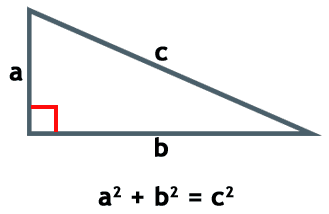
\includegraphics[width=0.8\textwidth]{pitagoras.png}
    \caption{La fórmula del teorema.}
    \label{fig:teo_pitagoras}
  \end{subfigure}
  \begin{subfigure}{0.45\textwidth}
    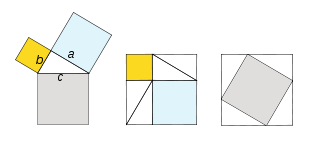
\includegraphics[width=1.0\textwidth]{pitagoras2.png}
    \caption{Demostración Gráfica del teorema.}
    \label{fig:grafica}
  \end{subfigure}
  \caption{Teorema de Pitágoras.}
\end{figure}

\section{Leyes de los Signos.}
\begin{table}[h]
  \centering
  \begin{tabular}{| c | c  | c |}
    \hline
    Operando & Operando & Resultado\\
    $+$  &  $+$  & $+$\\
    \hline
    $+$  &  $-$  & $-$\\
    \hline
    $-$  &  $+$  & $-$\\
    \hline
    $-$  &  $-$  & $+$\\
    \hline
  \end{tabular}
  \caption{Tabla con las leyes de los signos}
  \label{tab:leyes_signos}
\end{table}

\chapter{Jose Eduardo González Jasso}
\section{Mi descripcion.}
Me llamo Jose Eduardo voy a estudiar Ciencias de la computación en la Facultad de Ciencias. Elegí esta carrera pues me intersa aprendar a administrar Bases de Datos y porque a mi parecer en un futuro cercano las computadoras y en general los aparatos inteligentes formaran parte de la vida cotidiana de las personas, por lo cual es vital saber manejarlos profundamente.

\section{Mis libros favoritos}
\begin{enumerate}
\item El señor de los anillos: Las dos torres ~\cite{torres}
\item El señor de los anillos: El retorno del rey ~\cite{retorno}
\item El señor de los anillos: La comunidad del anillo ~\cite{comunidad}
\end{enumerate}
  

\subsection{Hobbies.}
\begin{enumerate}
\item Escuchar música en especial de tipo Rock
\item Jugar videojuegos en mis horas libres
\item Pasear a mis perros en la noche
\end{enumerate}

\begin{figure}[h]
  \centering
  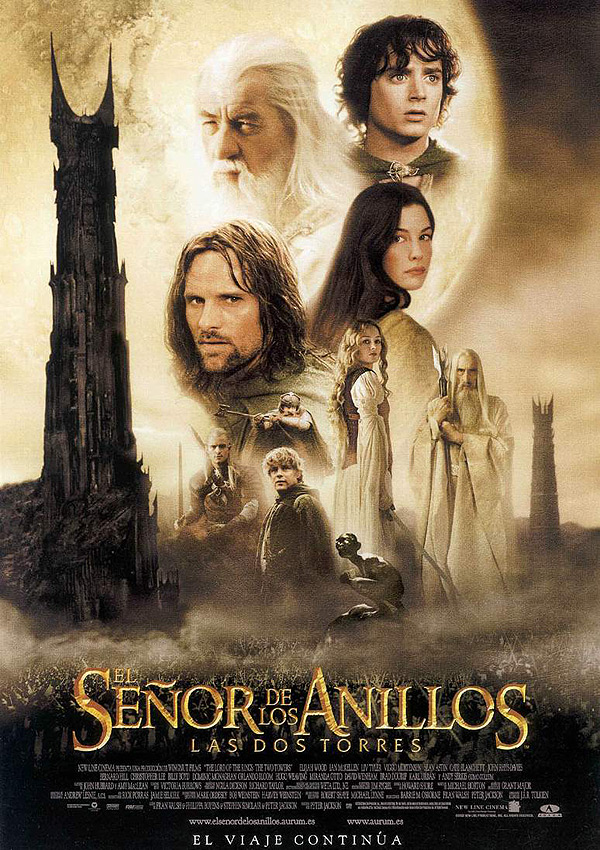
\includegraphics[scale=0.4]{IMG/13.jpg}
  \caption{Imagen de mi banda favorita}
  \label{fig:Soda}
\end{figure}

Podemos ver un ejemplo de una banda latinoamericana \textbf{\textbf{\emph{Figura}}}~\ref{fig:Soda}.

\newpage
Algunas formulas importantes en mi voda son:
\begin{itemize}
\item $c^2 = a^2 + b^2$
\item $x=-b \pm \frac{\sqrt{b^2-4ac}}{2a}$
\end{itemize}  
  
\section{Algo de matemáticas simples}

\begin{table}[h]
  \centering
  \begin{tabular} {| c c c |}
    \hline
    Operando & Operando & Resultado\\
    $+$ & $+$ & $+$\\
    $+$ & $-$ & $-$\\
    $-$ & $-$ & $-$\\
    $-$ & $+$ & $-$\\
    \hline
  \end{tabular}
  \caption{Leyes de los signos}
  \end{table}

\chapter{Alejandro Hernández Cano}

\section{Sobre mi}
Me llamo Alejandro y estoy cursando el propedeutico de Ciencias de la
Computacion en la Facultad de Ciencias de la UNAM.

\begin{figure}[h]
  \centering
  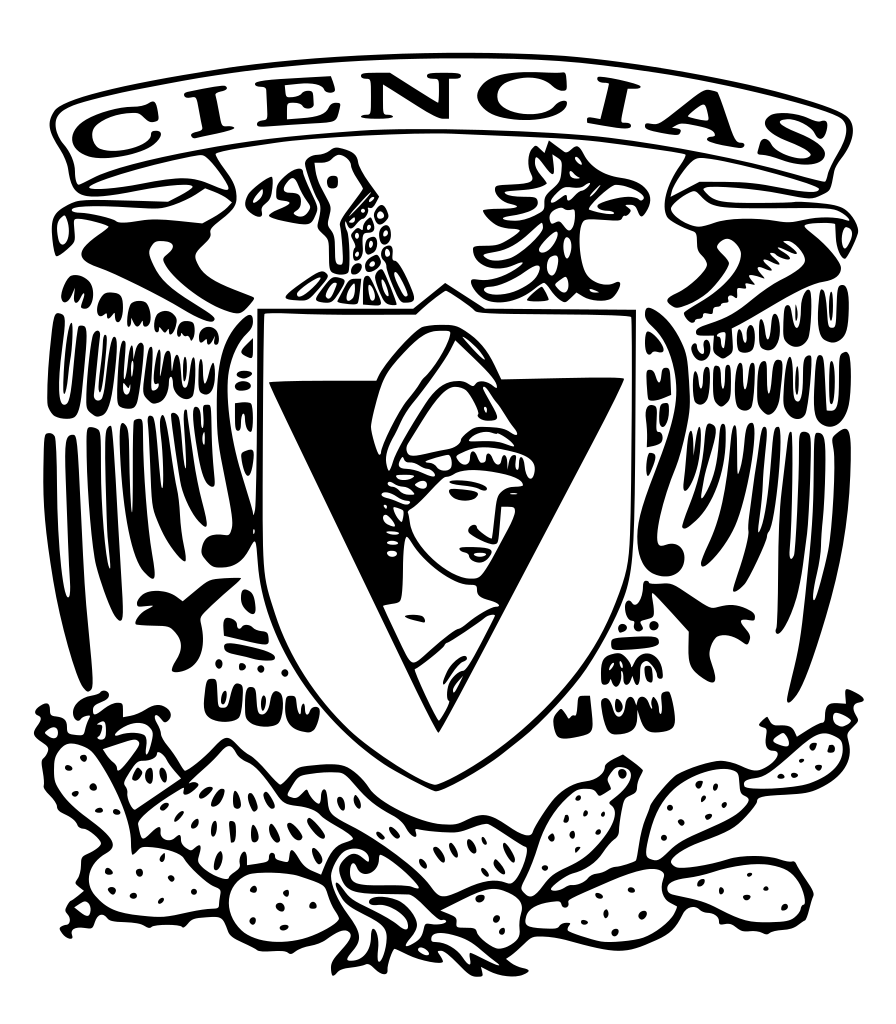
\includegraphics[scale=0.25]{3.png}
  \caption{Logo de la facultad de ciencias}
  \label{fig:fciencias}
\end{figure}

Podemos ver un ejemplo del logo de la facultad de ciencias en la
\emph{\textbf{figura}}~\ref{fig:fciencias}

\subsection{Hobbies}
Mis hobbies incluyen:
\begin{enumerate}
\item Escuchar música
\item Jugar videojuegos
\item Leer los libros ~\cite{torres, comunidad, retorno}
\end{enumerate}

\section{A profundidad}
Mucha gente se preguntará por qué decidí estudiar ciencias de la
computación. Este tema lo aboradré en las siguientes secciones
\subsection{Antecedentes}
Me gusta programar y me interesan las matemáticas.

\subsection{Las razones}
\begin{enumerate}
\item Me gusta programar
\item Me interesan las matemáticas
\end{enumerate}

\newpage
\section{Conocimientos}
\subsection{Leyes de los signos}
La \emph{\textbf{tabla}}~\ref{tab:signos} representa las leyes de los signos

\begin{table}[h]
  \centering
  \begin{tabular}{ c c c }
    Operando I & Operando II & Resultado\\
    \hline
    $+$ & $+$ & $+$\\
    $+$ & $-$ & $-$\\
    $-$ & $+$ & $-$\\
    $-$ & $-$ & $+$\\
  \end{tabular}
  \caption{Leyes de los signos}
  \label{tab:signos}
\end{table}

\subsection{Fórmulas importantes}
Algunas fórmulas importantes de mi vida son:
\begin{itemize}
\item $c^2 = a^2 + b^2$
\item $x = \frac{-b\pm\sqrt{b^2 - 4ac}}{2a}$
\end{itemize}

\section{Outro} 
\subsection{Agradecimientos}
Para el desarrollo de este libro, me gustaría hacer agradecimientos especiales
a los siguientes:
\begin{enumerate}
\item Mi familia
\item Mis maestros
\item Mis amigos
\item El lector
\end {enumerate}

\subsection{Palabras finales}
Este titulo tardó mucho tiempo en pensarse, desarrollarse, editarse e
inspeccionarse. Se ha llevado muchos tests de control para asegurarse de la
calidad del producto. Agradecemos su atención y ya.


\chapter*{Ulrich Villavicencio Cárdenas}

\section{Un poco sobre mí}

Me llamo Ulrich, tengo 17 años, entré a la carrera de Ciencias de la computación por medio del pase reglamentado.\\

\subsection{Hobbies}

\begin{enumerate}

  \item Deporte
  \item Leer
  \item Escuchar música
  
\end{enumerate}


\chapter{Shai Lèger Hernández}
	
	\begin{figure}[h]
		\centering
		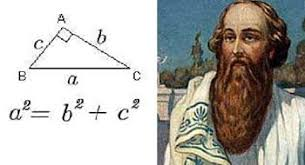
\includegraphics[scale=1]{./IMG/5.png}     
		\caption{Imagen de prueba}
		\label{fig:prueba}
	\end{figure}

\section{Sobre mi}

     - Tengo 18 años, tengo nacionalidad Canadiense, mi apellido es francés, mi nombre es hebreo.
     
\section{Hobbies}

	\begin{itemize}
		\item Programación
		\item Piano
	\end{itemize}
	
%referencias
%El \textbf{Teorema}-\ref{fig:prueba}

\newpage
\chapter{Cosas de matemáticas}

\section{Formulas}

	\begin{itemize}
		\begin{huge}
			\item {$c^{2} = a^{2} + b^{2}$}\\
			\item {$x =\frac{-b \pm \sqrt{b^{2} - 4ac}}{2a}$}\\
		\end{huge}
	\end{itemize}


\section{Tabla de ley de los simbolos}

	\begin{table}[h]
		\centering
		
		\label{tab:leyes_signos}
		\begin{tabular}{ | c | c | c | }
			
			\hline
			Operando & Operando & Resultado\\
			\hline
			$+$ & $+$ & $+$\\
			$+$ & $-$ & $-$\\
			$-$ & $+$ & $-$\\
			$-$ & $-$ & $+$\\
			\hline
			
		\end{tabular}
		\caption{Tabla de signos}
	\end{table}
	
	\centering\emph{Plantilla para hacer una \emph{Tabla}~\ref{tab:leyes_signos} en \LaTeX}
		



\chapter{Alexia}

\section{un poco sobre mi}
\textbf{ADVERTENCIA. Lees esto a conciencia de que son tonterias.}

Me llaman Alexia, realmento solo aspiro a la felicidad, ya lo se, super cliche pero pues...me gusta, voy en la facultad de ciencias, porque, no es que sea especialmente buena, de hecho no lo soy, pero vale la pena seguir, es divertido :) ahhh y vengo de prepa 9, tome alguna clase de programacion c++ y pues me gusto, así que aquí estoy. 


Me gusta mucho leer los libros~\cite{torres,comunidad,retorno}

\subsection{hobbies}

\begin{enumerate}
\item cantar
\item respirar (hacer yoga y ballet)
\item tocar el piano
\end{enumerate}

\begin{figure}[h]
  \centering
  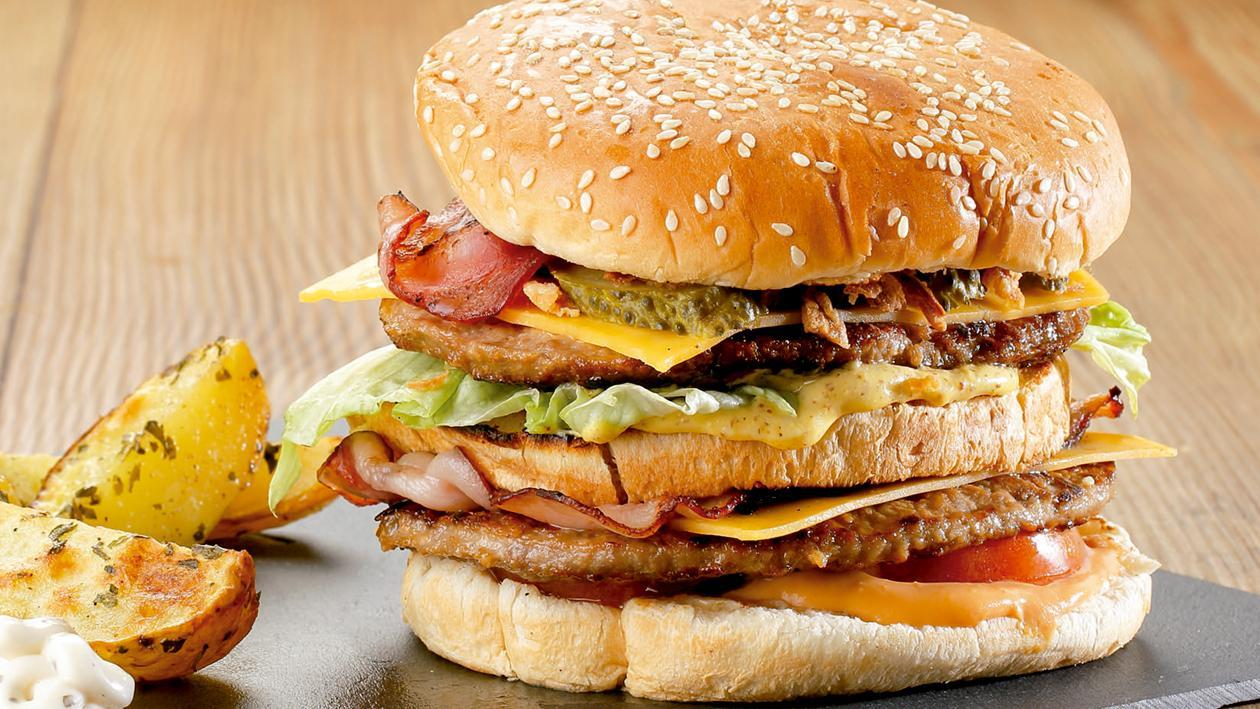
\includegraphics[scale=0.10]{IMG/6.jpg}
  \caption{my love}
  \label{fig:hamburguesa}
\end {figure}

Podemos ver una deliciosa hambueguesa llamada comunmente por mi: amor
\textbf{figura}~\ref{fig:hamburguesa}.

\begin{itemize}
\item $c^{-ba}$
\item $x=-b_a \pm \frac{5}{\sqrt{9}}$
 \end{itemize}

\begin{tabular}{|l | c | r|}
  \hline
  comida & yet & porcino \\
  \hline
  pepinillos & gorra & carpa \\
  \hline
  
\end{tabular}


\chapter{Karla}

\section{Un poco sobre mi}
Mi nombre es Karla Denia (\textbf{\emph{Figura de Poblado Denia en España}}~\ref{fig:Dénia}), tengo 18 años, estudie en la ENP6, me gusta programar desde la secundaria, pero fue hasta la carrera técnica en computación que decidí que ciencias  erami mejor opción y pues aquí estoy, tratando de no morir en el intento. Mi mayor sueño es viajar por todo el mundo.
\begin{figure}[h]
  \centering
  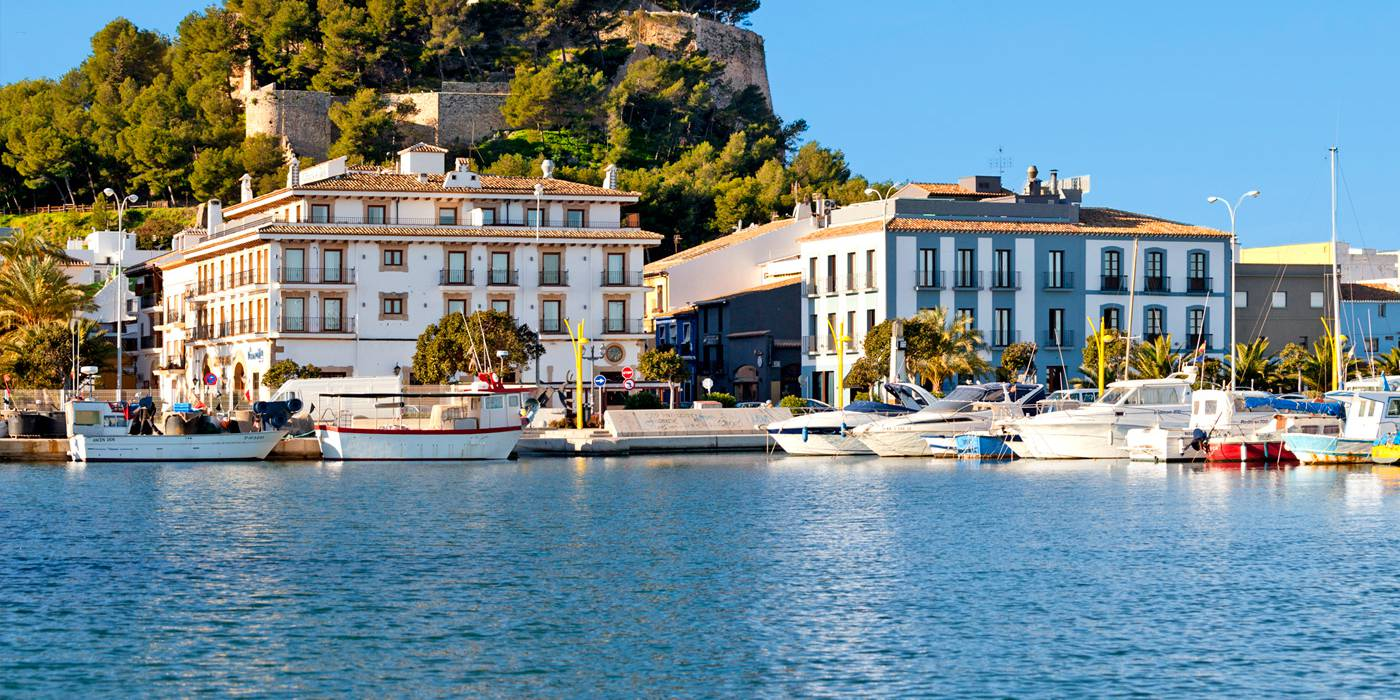
\includegraphics[scale=0.15]{IMG/7.jpg}
  \caption{Dénia, España}
  \label{fig:Dénia}
\end{figure}
\subsection{Hobbies}
\begin{itemize}
\item Jugar voleibol
\item Leer~\cite{torres,comunidad,retorno}, sobretodo en el transporte público
\item Escuchar música, mi instumento favorito es el violín.
\end{itemize}
\begin{figure}[h!]
  \centering
  {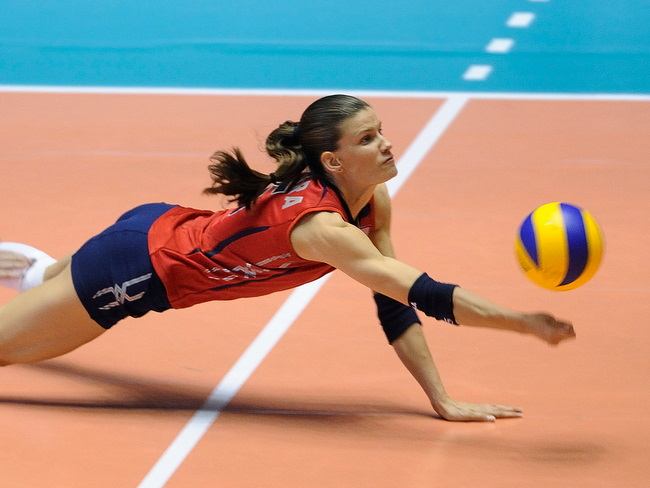
\includegraphics[scale=0.25]{IMG/7_2.jpg}}
  {
\includegraphics[scale=0.29]{IMG/7_3.jpg}}
  {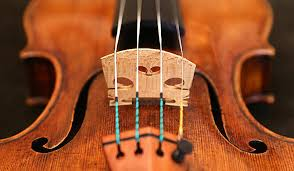
\includegraphics[scale=0.54]{IMG/7_4.jpg}}
  \caption{Hobbies}
\end{figure}



\maketitle

\listoffigures
\addcontentsline{toc}{chapter}{Índice de figuras}


\chapter*{Jose Ignacio Hernandez Valle}


\chapter{Ignacio mi historia}
\section{Un poco sobre mi}

Me llamo Ignacio y soy estudiante de Ciencias de la Computacion naci en la Ciudad de Mexico tengo 20 años
Entre a esta carrera por medio de examen, para este llevo preparandome muchos meses ya que para entrar la cantidad de aciertos que piden es muy alta, estudie en la Prepa 6 pero tuve problemas en sexto año en la materia de quimica esto no me permitio concluir mi bachillerato ahí, para lograr tener mi certificado estuve inventigando las maneras que se ofrecen para concluir el bachillerato gracias a esto encontre el ``Examen Unico'' de Colegio de Bachilleres y logre terminar la preparatoria

\subsection{Hobbies}
\begin{enumerate}
  
\item Hacer ejercicio
\item Andar en moto y bicicleta
\item Escuchar musica
\end{enumerate}

\begin{figure}[h]
  \centering
  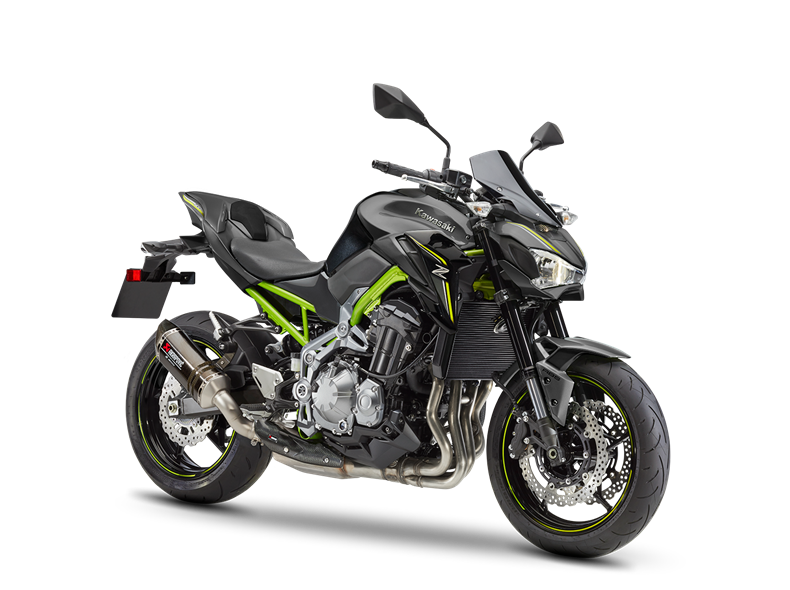
\includegraphics[scale=0.5]{IMG/8_1.png}
  \caption{\small Kawasaki z900 mi moto soñada} \label{fig:8_1}
\end{figure}

\begin{figure}[h]
  \centering
  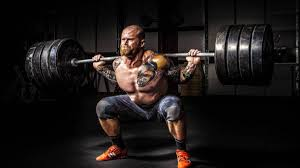
\includegraphics[scale=0.8]{IMG/8_2.jpg}
  \caption{\small Fitness } \label{fig:8_2}
\end{figure}



\chapter{Berenice Calvario Gonzalez}
\section{Un poco sobre mi}
Me llamo Berenice y soy estudiante de Ciencias de la Computación. 

\subsection{Hobbies}
\begin{enumerate}
\item Tocar el violín y el piano
  
  \begin{figure}[h]
    \centering
    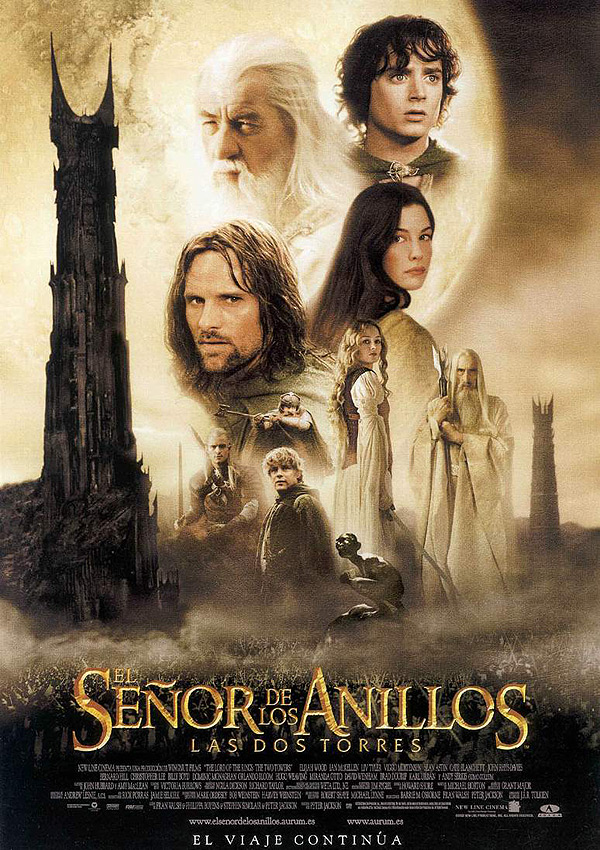
\includegraphics[scale=0.02]{IMG/13.jpg}
    \caption{\small partitura} \label{fig:1}
  \end{figure}

  
      
\item Nadar

  \begin{figure}[h] 
    \centering
    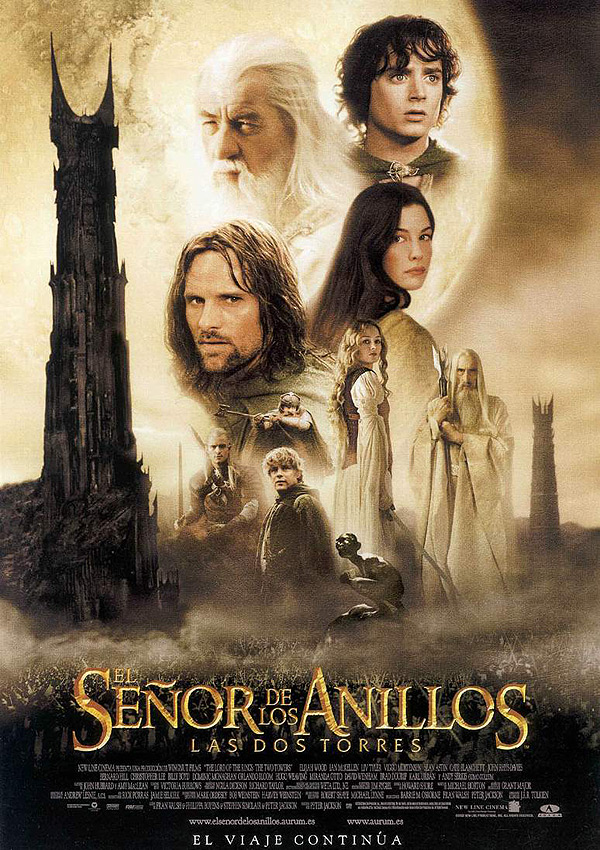
\includegraphics[scale=0.5]{IMG/13.jpg}
    \caption{\small nadar} \label{fig:2}
  \end{figure}
  
\item
\end{enumerate}

\begin{table}[h]
  \centering
  \begin{tabular}{ c c c }
    \hline
    operando & operando & resultado\\
    $+$ & $+$ & $+$\\
    $+$ & $-$ & $-$\\
    $-$ & $+$ & $-$\\
    $-$ & $-$ & $+$\\
    \hline
  \end{tabular}
\end{table}

\chapter{Claudia Osorio Lopez}

\section{Algo Sobre mi:}
Me llamo Claudia, tengo 18 años. Vivo en Pedregal de San Nicolas. Estudie en CHH Sur y elegi la carrera de Ciencias de la Computacion en la Facultad de Ciencias en Ciudad Universitaria.

Me gusta leer~\cite{Floodlight,Tokuyama}


\subsection{Hobbies}
Entre mis hobbies estan:
\begin{enumerate}
  \item{Escuchar Musica
  \item{Leer
  \item{Limpiar
  \item[Caminar
\end{enumerate}

\begin{figure}[h]
  \centering
  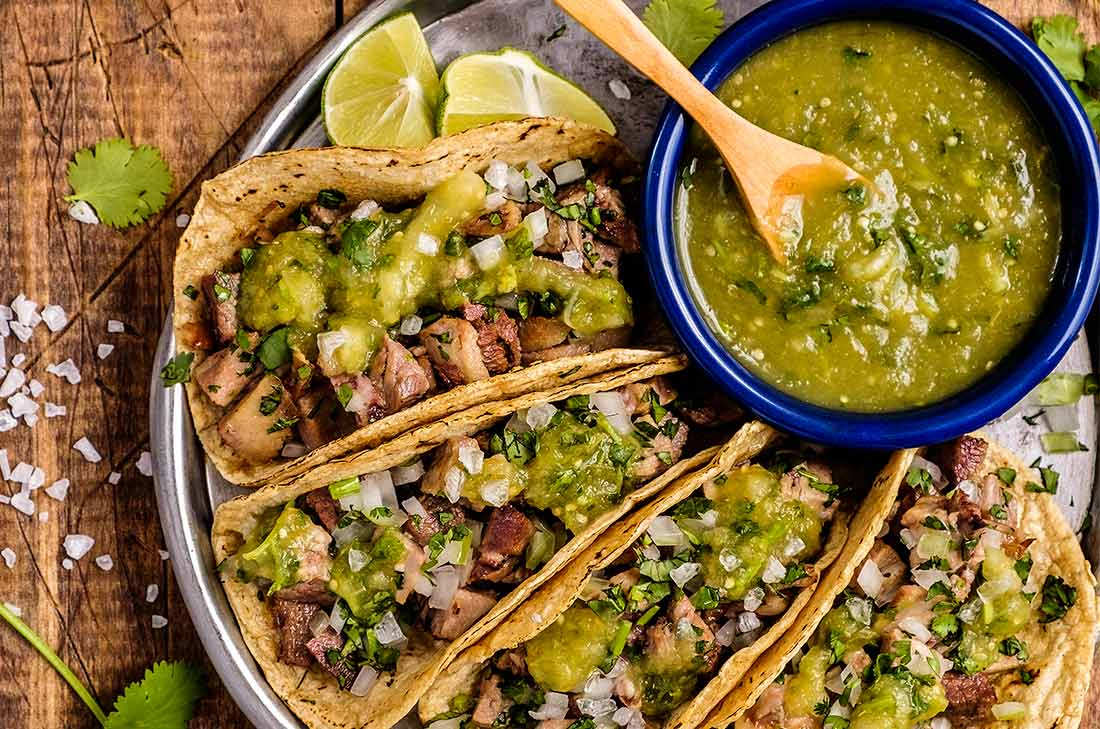
\includegraphics[scale=0.2]{IMG/tacos.jpg}
  \caption{De mis comidad favoritas}
  \label{fig:tacos}
\end{figure}

\chapter{Alejandro Blancas Peralta}

\section{Algo Sobre mi:}
Me llamo Alejandro, tengo 18 años. Vivo en Cuautepec. Estudie en CHH Vallejo, estudiaré la carrera de Ciencias de la Computacion en la Facultad de Ciencias en Ciudad Universitaria.
 Leo:~\cite{comunidad,torres,retorno}

\subsection{Hobbies}
Entre mis hobbies estan:

\begin{enumerate}
  \item{Jugar Videojuegos
  \item{Dibujar
  \item{PvZx
\end{enumerate}

\begin{figure}[h]
  \centering
  
\includegraphics[scale=0.2]{IMG/Girasol_.jpg}
  \caption{\small algo sobre eso} \label{fig:Girasol_}
\end{figure}
x
Podemos ver en la imagen anterior un hermoso girasol en la
\emph{\textbf{figura}}~\ref{fig:Girasol_}

\begin{table}[h]
  \centering
  \begin{tabular}{| c | c | c |}
    \hline
    Operando & Operando & Resultado\\\hline
    $+$ & $+$ & $+$\\\hline
    $+$ & $-$ & $-$\\\hline
    $-$ & $+$ & $-$\\\hline
    $-$ & $-$ & $+$\\\hline
    \hline
  \end{tabular}
\end{table}

\newpage
Algunas formulas importantes de la vida son:
\begin{itemize}
  \item $c^{2} = a^{2} + b^{2}$
  \item $X= -b \pm \frac{\sqrt{b^{2}-4ac}}{2a}$
    \end{itemize}

\include{capitulo12}

\chapter{Vladimir Sierra}



\section{Un poco sobre mí}

Tengo 18 años, me llamo Vladimir, nací y viví hasta los 15 años en TLapa Guerrero.
Durante toda mi vida he sentido gran pasión por las Matemáticas; también me interesan mucho las artes, toco guitarra y piano. Siempre he querido aprender a pintar pero creo que no es algo en lo que sea bueno.
Mis gustos musicales son un poco variados, pero creo que el género que más me deleita escuchar es la trova.
SI pudiera resumir mis gustos diría, que mi músico favorito es SIlvio Rodríguez, escritor favorito es Haruki Murakami, y pintor favorito quizá sea Francisco de Goya.
También me interesa mucho el fútbol, antes solía jugar, pero a partir de que las obligaciones en la escuela se volvieron más pesadas lo deje.
Acabo de ingresar a la Facultad de Ciencias para estudiar Ciencias de la Computación.

Haruki Murakami es de mis autores favoritos, entre mis libros favoritos de él están 

\subsection {hobbies}
\begin{enumerate}
\item Tocar guitarra
\item Jugar soccer
\item Leer
\item Estudiar Matemáticas
\end{enumerate}  

Escogí la carrera porquer: 


\begin{itemize}
\item Me gustan las estructuras
\item Me gusta resolver problemas
  \item Soy bueno en Análisis Matemático
 \end{itemize}

\newpage

    \section{Películas favoritas}
    Mis trilogía favorita es sin duda la del Señor de los anillos, pero algo que tengo pendiente por hacer es leer los libros~\cite{torres,comunidad,retorno}
    
\begin{figure}[h]
\centering
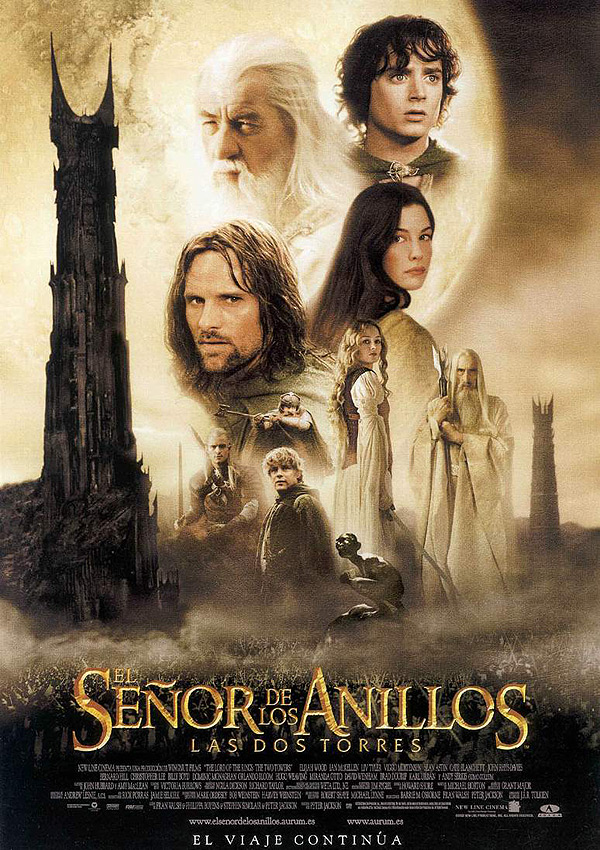
\includegraphics[scale=0.5]{IMG/13.jpg}
\caption {Adjunto imagen de una portada}

\label{fig:anillos}
\end{figure}

Podemos ver una portada de una de las \emph{películas} en la \emph{\textbf{Figura}}~\ref{fig:anillo}



\chapter{Antonio Sebastian Dromundo Escobedo}

\section{Yo}
Soy Sebastian y soy estudiante de Ciencias de a computación en la Facultad de Ciencias :)

Solo he leido el primer libro del señor de los anillos ~\cite{comunidad}

\subsection{Hobbies}
\begin{enumerate}
\item Tocar la guitarra
\item Ver peliculas
\item Pasear
\end{enumerate}

3 cosas importantes para mi son

\begin{itemize}
\item Mi guitarra
\item Mi computadora
\item Mis fotos
\end{itemize}

\newpage
Just filling some space:
\begin{itemize}
\item $c^2 = a^2 + b^2$
\item $F_{e} = k \frac{q_{1} q_{2}}{r^2}$
\item $x= \frac{-b \pm \sqrt{b^2-4ac}}{2a}$
\end{itemize}

\section{This seems to be fun}
\begin{figure}[h]
  \centering
  
\includegraphics[scale=0.5]{IMG/Fry.jpg}
  \caption{Wubba Lubba Dub Dub}
  \label{fig:fry}
\end{figure}

Not quite sure what to cite so I'm just letting a photo af myself \emph{life} en la \emph{\textbf{Figura~\ref{fig:fry}.}}

\begin{table}[h]
  \centering
  \begin{tabular}{| c  c  c  |}
    \hline
    Proposicion 1 & Proposicion 2 &1 y  2 \\\hline
    $+$ & $+$ & $+$\\\hline
    $+$ & $-$ & $-$\\\hline
    $-$ & $+$ & $-$\\\hline
    $-$ & $-$ & $+$\\\hline    
  \end{tabular}
  \caption{Tabla de verdad de Conjuncion}
  \label{tabla:afirmaciones}
\end{table}

En la \textbf{\emph{Tabla}}~\ref{tabla:afirmaciones} el signo afirmativo se refiere a verdadero y el negativo a falso.



\author{jose  \thanks{josemigueltr@hotmail.com}}
\title{ Curso Propedeutico 2019 }
\date{\today}


\maketitle
\tableofcontents
\addcontentsline{toc}{chapter}{Índice}



\chapter{Miguel Toledo Reyes}


\section{un poco sobre mi}
 mi nombre es miguel, estudie en la Escuela Nacional Preparatoria No.1 ``Gabino Bareda'', Vivo actualmente en xochimilco.

\subsection{hobbies}
\begin{enumerate}
\item   Me gusta correr
\item   Jugar videojuegos
\item   Programar
\item   resolver problemas
 \end{enumerate}


\section{ carateristicas}
\begin{itemize}
\item    Alto
\item   Moreno
\item   Delgado
  \item  Pelo negro

  Este es el logo de la consola en la que juego videojuegos\\
  
  \begin{figure}[h]
  \centering
  
\includegraphics[scale=.5]{IMG/15.png}
  \caption{Logo de la consola en la que juego}
  \label{fig:Logo de xbox}
  \end{figure}



    
\begin{table}[h]
   Este es un ejemplo de las leyes de los exponentes\\
  \centering
  \begin{tabular}{| c | c | c | }
    \hline
    Operando & Operando & Resultado\\\hline
    $+$ & $-$ & $-$\\\hline
    $+$ & $-$ & $-$\\\hline
    $-$ & $-$ & $+$\\\hline
    $+$ & $+$ & $+$\\\hline
  \end{tabular}
  \caption{leyes de los signos}
  \label{tabla :leyes de los signos}
  \end{table}
Esta tabla la saque del libro~\cite{Floodlight}.




\newpage
Algunas formulas  importantes son:
\begin{itemize} 
\item La formula  pitagorica: $ c^2=a^2+b^2$  La formula de resolucion de ecuacionesde segudo grado:
\item $x=-b\pm\frac{\sqrt{b^2-4ac}}{2a}$
\end{itemize}



Plantilla de \LaTeX.\\

% https://www.lipsum.com
\section{Lorem ipsum}

Lorem ipsum dolor sit amet, consectetur adipiscing elit. Quisque lectus ligula,
tristique ut erat eu, elementum ullamcorper elit. Nullam vel aliquam neque, at
malesuada leo. Cras nec libero sed erat hendrerit dapibus. Vestibulum leo nunc,
condimentum sed viverra sollicitudin, convallis in arcu. Nulla a metus a libero
imperdiet rutrum. Proin fringilla purus quis sagittis tempus. Orci varius
natoque penatibus et magnis dis parturient montes, nascetur ridiculus mus. Lorem
ipsum dolor sit amet, consectetur adipiscing elit. Sed tristique mauris nec dui
pellentesque dapibus. Nulla facilisi. Etiam convallis venenatis mattis. Ut
facilisis maximus nulla, sed volutpat leo dignissim vitae. Integer at quam eget
nisl porttitor faucibus.

Duis bibendum tortor ac nisl scelerisque, quis gravida magna dictum. Aliquam vel
imperdiet leo, at hendrerit est. Donec porta feugiat metus nec fringilla. Nulla
nec odio in libero gravida volutpat. Sed ut lacus tristique, lacinia dolor at,
fringilla odio. Aliquam accumsan suscipit diam id imperdiet. Pellentesque vitae
tempus arcu. Etiam a dapibus nibh, sit amet finibus ipsum. Nunc ac mollis
nibh. Donec vel nibh ac lectus pellentesque viverra.

Cras sollicitudin ac nulla at lobortis. Nullam finibus quam tortor, vel semper
ligula semper et. Ut nec ultrices odio, eu facilisis turpis. In ut facilisis
enim. Mauris sit amet ex vitae ante commodo volutpat at ut ipsum. Donec
condimentum sed enim sit amet molestie. Mauris mauris neque, tincidunt eu rutrum
finibus, commodo euismod augue. Donec non diam eu augue lobortis iaculis. Duis
hendrerit, ligula ut pulvinar ullamcorper, ligula lacus viverra justo, non
sagittis dui augue viverra augue. Praesent convallis placerat nisi in
sodales. Donec a rhoncus leo. Mauris porta leo semper tellus tempus
molestie. Aliquam vel eros cursus, elementum metus a, dictum felis. Nunc sed
tortor convallis justo aliquam dapibus eget sollicitudin mi.

Cras in enim risus. In venenatis feugiat lectus, ac malesuada arcu aliquet
ac. Quisque vitae ante ipsum. Fusce vitae tortor lectus. Pellentesque commodo
ligula vitae leo ultrices tempor. Proin id purus vitae risus rutrum dapibus ut
ac enim. Duis porttitor, massa eu dignissim fermentum, turpis augue consectetur
nulla, eu porta lorem augue ac lacus.

Sed in aliquam magna. Cras nec leo augue. Nulla pellentesque fermentum
massa. Nulla eget eros id nisi pretium vestibulum id nec lacus. Integer euismod
dolor vitae pharetra fermentum. Nulla hendrerit massa et magna lobortis
porttitor. Donec venenatis commodo erat ut dignissim. Quisque vestibulum eros
mollis libero pulvinar tristique et in nisl. Quisque finibus feugiat purus,
vehicula aliquam mi malesuada molestie.





\chapter{Diego Jardon}
\paragraph{
  13 de septiembre de 1999, yo nazco en un pueblo de estos de Guerrero pero me mudo a Michoacán por decisión de mi padre a los 4 años de edad, donde viví mi niñez y la mayor parte de la adolescencia, hoy (no precisamente hoy), me mudo a la Ciudad de México para estudiar en la Universidad Nacional Autonoma de Mexico.
}

\section{Hobbies:}

\begin{itemize}
    \item{Hacer Parkour}
    \item{Programar}
    \item{Caminar}
    \item{Leer \cite{cita}}
\end{itemize}

\begin{figure}[h]
  \centering
  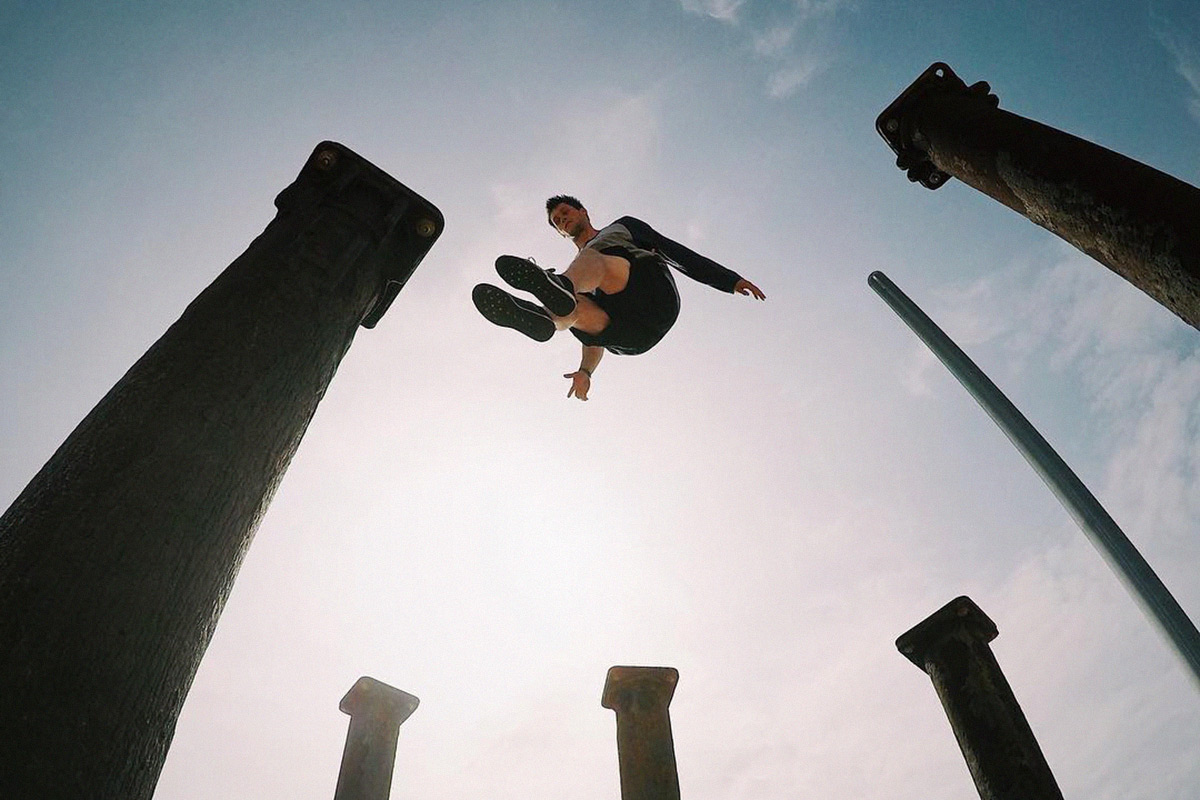
\includegraphics[scale=0.15]{IMG/1.jpg}
  \caption{Parkour}
\end{figure}
\chapter{José Luis García Santamaría}

\section{un poco sobre mi}
Acabo de entrar a la carrera de ciencias de la computacion, provengo del cch sur y elegi la carrera porque me parecio mas completa que la ingenieria en sistemas

\subsection{hobbies}
\begin{enumerate}

\item hobbie Nadar

  \begin{figure}[h]
    \centering
    
\includegraphics[scale=0.5]{IMG/17.jpg}
  \end{figure}

\item hobbie Ver Youtube

  \begin{figure}[h]
    \centering
    
\includegraphics[scale=0.5]{IMG/17.jpg}
    \caption{Viendo Youtube}
  \end{figure}
  
\item hobbie Me gusta escuchar musica

  \begin{figure}[h]
    \centering
    
\includegraphics[scale=0.5]{IMG/17_2.jpg}
    \caption{Escuchando musica}
  \end{figure}
  
\end{enumerate}



\chapter{Juan García Lugo}

% https://www.lipsum.com
\section{Un poco soobre mí}

Yo nací el 5 de enero del 2000, soy hombre, vengo de una familia nuclear, tengo muchos familiares que viven muy cerca de mi casa, tengo varios amigos, y una novia, me gusta mucho las matemáticas, la física , y la computación (más las matemáticas, hasta ahora), me gusta mucho el pan, tengo una complexión delgada, mido 1,68, peso 63 kilogramos, uso lentes, por lo regular tengo el cabello largo, pero ahora por motivos de la cartilla militar, me lo corte, y pues me gusto el corte.

\begin{figure}[h]
  \centering
  
\includegraphics[scale=0.125]{IMG/18.jpg}
  \caption{García Lugo Juan}
  \label{foto:juan}
\end{figure}

El chico que esta arriba \emph{\textbf{soy yo}}~\ref{foto:juan} a los 16   
\section{¿Porque elegí esta carrera?}

La carrera la elegí, porque me gusto mucho, la gran capacidad de los programadores, para generar algoritmos, y encontrar soluciones computables, a ciertos problemas, y de por si , la carrea en genral me parece muy interesante


\section{¿Qué me gusta hacer?}

\begin{enumerate}
\item Estudiar
\item Leer
\item Hacer ejercicio
\item resolver ejercicios
\item caminar
\end{enumerate}

\section {Lo que nunca me aprendi}

\begin{table}[h]
  \centering
  \begin{tabular} {c c c}
    \hline
    operando & operando & Resultado\\

    $+$ & $+$ & $+$\\
    $+$ & $-$ & $-$\\
    $-$ & $+$ & $-$\\
    $-$ & $-$ & $+$\\

    \label{No}
    
  \end{tabular}
\end{table}

nunca me aprendí \emph{\textbf{ Las leyes de los signos}}~\ref{No}, pero siempre tengo conmigo una tabla que me ayuda a recordarlos

\chapter{Breve historia de mi vida}

Hola soy Martin, actualmete  fui aceptado en la facultad de Ciencias en la carrera de Ciencias de la computacion, naci el 9 de agosto de 1999, y he pasado casi toda mi vida en la Ciudad de México a ecepción de un par de años que viví en púebla

\begin{figure}[h]
  \centering
  
\includegraphics[scale=0.5]{IMG/19_2.jpg}
  \caption{Facultad de ciencias}
  \label{fig:facultad}
\end{figure}


\chapter*{Mi familia}

Mi padre se llama MIguel Ángel, y mi madre se llama Sandra Lisbeth; Tengo 2 hermanos, mi hermano mayor se llama Josue y mi hermana menor se llama Ana

\begin{figure}[h]
  \centering
  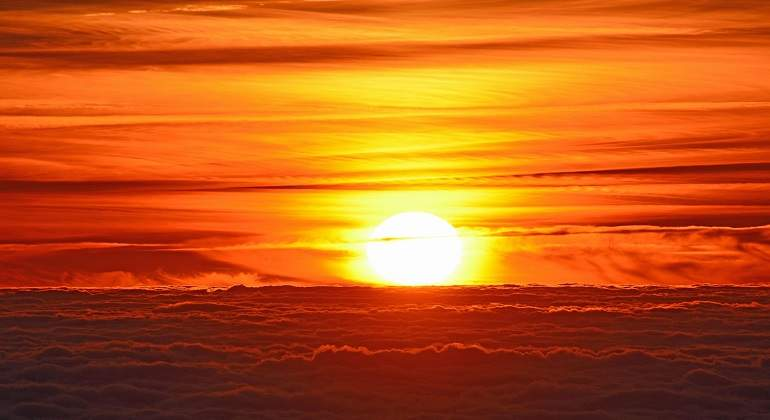
\includegraphics[scale=0.5]{IMG/19_4.jpg}
  \caption{Atardecer}
  \label{fig:atardecer}
\end{figure}


\chapter*{Mis gustos}

Me gustan las matemáticas ya que son bastantes entretenidas y en ellas encuentro muchos retos interesantes
\begin{itemize}
\item $c^2 = a^2 + b^2$
\item $x=-b \pm \frac{\sqrt{b^2-4ac}}{2a}$
\end{itemize}


\begin{table}[h]
  \centering
  \begin{tabular}{| c  c  c  |}
    \hline
    Operando & Operando & Resultado\\\hline
    $+$ & $+$ & $+$\\\hline
    $+$ & $-$ & $-$\\\hline
    $-$ & $+$ & $-$\\\hline
    $-$ & $-$ & $+$\\\hline    
  \end{tabular}
  \caption{Leyes de los signos}
  \label{tabla:leyes_signos}
\end{table}

Tambien me agrada bastante la música del anterior siglo
\begin{figure}[h]
  \centering
  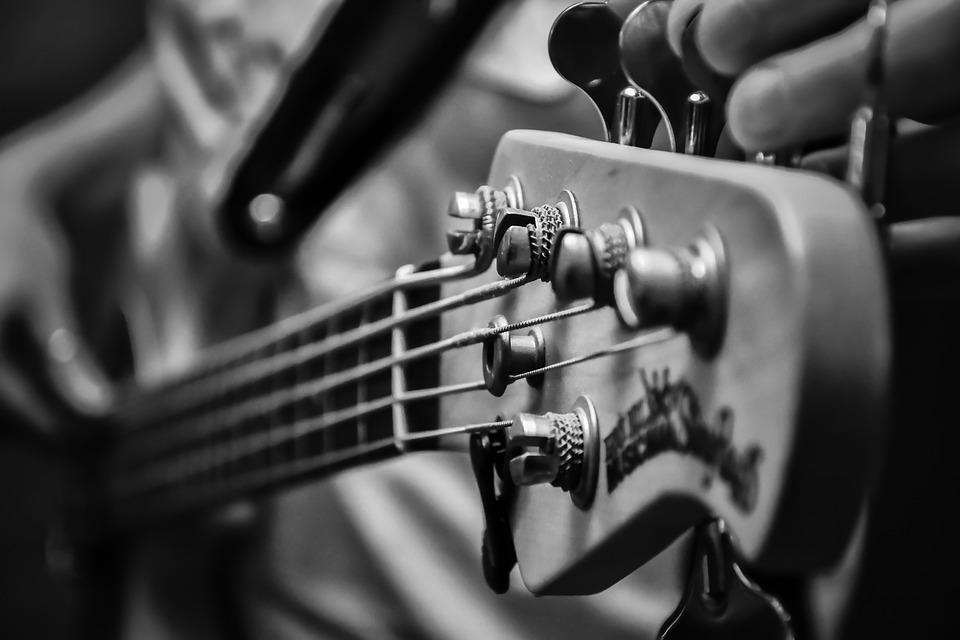
\includegraphics[scale=0.5]{IMG/19_1.jpg}
  \caption{iamgen de lo que me gustaria aprender}
  \label{fig:guitarra}
\end{figure}

\chapter{Mis planes}

Planeo terminar mi carrera, conseguir un buen empleo, administrar mi tiempo para continuar con estudios de pos grado, e intentar ser feliz-

\begin{figure}[h]
  \centering
  
\includegraphics[scale=0.5]{IMG/19_3.jpg}
  \caption{ciencias de la computacion}
  \label{fig:computo}
\end{figure}







\author{Miguel Angel Reyes}
\title{Mi bio}
\date{\today}

\renewcommand{\labelitemi}{$\bullet$}


\begin{document}

\maketitle
\tableofcontents
\addcontentsline{toc}{chapter}{Índice}

\listoffigures
\addcontentsline{toc}{chapter}{Índice de figuras}

\listoftables
\addcontentsline{toc}{chapter}{Índice de tablas}

\chapter*{Introducción}

Bueno aqui tendria que poner algo solo que no se me ocurre algo asi que voy a iniciar :(
\chapter{Miguel Angel}

\section{Un poco sobre mi}
Mi nombre completo es Miguel Angel Reyes Encarnacion, estoy estudiando la carrera de ciencias de la computacion

Mi trabajo de tesis estuvo basado en el artículo~\cite{Floodlight}.

Me gusta mucho leer los libros (estos no son a mi me gusta el terror mas stephen king)~\cite{torres,comunidad,retorno}

\subsection{Hobbies}
Mis hobbies son:
\begin{enumerate}
\item Leer
\item Jugar Videojuegos
\item Generalmente ve peliculas, la mayoria de terror
\end{enumerate}

\newpage
Algunas fórmulas importantes en mi vida son:
\begin{itemize}
\item $c^2 = a^2 + b^2$
\item $x=-b \pm \frac{\sqrt{b^2-4ac}}{2a}$
\end{itemize}

\section{Libro}
\begin{figure}[h]
  \centering
  
\includegraphics[scale=0.5]{IMG/20.jpeg}
  \caption{Imagen de un Libro}
  \label{fig:Libro}
\end{figure}

Podemos ver un ejemplo del \emph{Teorema de Pitagoras} en la
\emph{\textbf{Figura}}~\ref{fig:Libro}.


\begin{table}[h]
  \centering
  \begin{tabular}{| c  c  c  |}
    \hline
    Operando & Operando & Resultado\\\hline
    $+$ & $+$ & $+$\\\hline
    $+$ & $-$ & $-$\\\hline
    $-$ & $+$ & $-$\\\hline
    $-$ & $-$ & $+$\\\hline    
  \end{tabular}
  \caption{Leyes de los signos}
  \label{tabla:leyes_signos}
\end{table}

Yo aprendí las leyes de los signos en la secundaria, tal como
se muestra en la \textbf{\emph{Tabla}}~\ref{tabla:leyes_signos}.

Bueno como veran copie todo, en realidad no se si puse todo bien pero espero que lo hayan disfrutado

\chapter{Oscar}

\section{Introduccion}
When todo empezo.... 
ashfbasiuhfaisjdhfiasd
asfjhbasldkjfljbaISBISABFSALJKBFOUIEASBEFLKSJDBFSIHDBFESWGsadnfijasbdnfouiasbhfjksnbdvlkjsdabvljkdsbvlkjsbdfvljidbsgvlkajdbv

\section{Un poco sobre mi}
Me llamo juan perez y me gusta la pizza
Me interesa la lectura ~\cite{guerra,hombre,ensayo,orwel,huxley}

\section{La historia de mi vida}
Era hace una vez en una galaxia muy lejana............... 

\subsection{Hobbies}
\begin{enumerate}
\item Badminton
\item Basket
\item Anime
\item Morritas de 15
\item Gatitos
\item Mapaches
\item Chocolate
\end{enumerate}
Me gusta mirar el atardecer y las largas caminatas por la playa :V

\subsection{Otras cosas}
\begin{itemize}
\item Mengo hambre
\item Me gusta el pan
\item Holi boli crayoli
\end{itemize}

\begin{figure}
  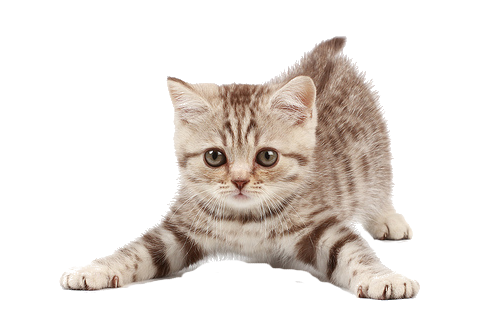
\includegraphics[scale=0.25]{21.png}
  \caption{Imagen de un gatito <3 }
  \label{fig:Gatito}
\end{figure}

\section{Matematicas}
Algunas formulas mamalonas:
\begin{itemize}
\item $c^2 = a^2 + b^2$  
\item $x = -b \pm \frac{\sqrt{b^2-4ac}}{2a}$
\end{itemize}

Aqui podemos ver una tabla mamalona ;v
\emph{\textbf{Tabla}}~\ref{tab:Signos}

\begin{table}[h]
  \centering
  \begin{tabular}{| c | c | c |}
    \hline
    Operando & Operando & Resultado\\\hline
    $+$ & $+$ & $+$\\\hline
    $+$ & $-$ & $-$\\\hline
    $-$ & $+$ & $-$\\\hline
    $-$ & $-$ & $+$\\\hline    
  \end{tabular}
  \caption{Signos}
  \label{tab:Signos}
\end{table}


Podemos ver un lindo gatito
\emph{\textbf{Figura}}~\ref{fig:Gatito}

\chapter{Azul}
Me llamo Azul y tengo el cabello rosa.

\section{Hobbies}

\begin{enumerate}
\item ver vídeos en YouTube
\item tocar el violín
\item aprender japonés
\end {enumerate}

\section{Información}

\begin{itemize}
\item Soy de la CDMX
\item Tengo 19 años
\item Entré por examen de selección
\item Me interesa el diseño web
\end{itemize}

\section{Formulas}
Algunas fórmulas importantes en mi vida son:
\begin{itemize}
\item $c^2=a^2+b^2$
\end{itemize}
  
\begin{table}[h]
  \centering
  \begin{tabular}{|c c c|}
    \hline
    Operando & Operando & Resultado\\
    $+$ & $+$ & $+$\\\hline
    $+$ & $-$ & $-$\\\hline
    $-$ & $+$ & $-$\\\hline
    $-$ & $-$ & $+$\\\hline
\end{tabular}
\end{table}

\section{Libros}
Los libros que me gustan son~\cite{salinger2001guardian, rice2014entrevista, shelley2008frankenstein, marias2011corazon}

\begin{figure}[h]
  \Centering
  \Includegraphics[scale=0.5]{img/22.png}
  \caption {violin}
  \label{fig:violin}
\end{figure}

Podemos ver un ejemplo de un violin en
\emph{\textbf {violín}}~\ref{fig:violin}
\chapter{Emiliano}
Me llamo Emiliano, tengo 18 años y vivo en Xochimilco

\section{Hobbies}

\begin{enumerate}
\item ver vídeos en YouTube
\item tocar la guitarra
\item jugar videojuegos
\end {enumerate}

\section{Información}

\begin{itemize}
\item Soy de la CDMX
\item Estudie en Prepa 5
\item Me interesa la programacion
\end{itemize}

\chapter{Mauricio Riva Palacio Orozco}

\section{Un poco sobre mi}
Me llamo Mauricio y soy estudiante de primer ingreso en ciencias de la computacion, me gusta escuchar música y salir 

\subsection{Hobbies}
Me gustan los deportes como el tennis, el futbol americano, etc. 

\section{Porque ciencias de la computacion?}
Porque es lo que me gusta y tengo muchas ganas de aprender

\subsection{Imagenes}
Una imagen de prueba

\begin{figure}[b]
  \centering
  
\includegraphics[scale=0.5]{IMGA/linux.png}
  \caption{Imagen sobre linux}
\end{figure}

\include{capitulo25}
\chapter{Sebastián Alamina Ramírez}

\section{About me.}
Me llamo Sebastián, tengo 18 años y voy a estudiar Ciencias de la Computación en la Facultad de Ciencias de la UNAM (\textbf{Figura \ref{fig:26}}). Además puedo confirmar que tuvimos un susto de alerta en el último día del curso propedéutico, tal como se menciona en la introducción del libro.

\begin{figure}[h]
\centering
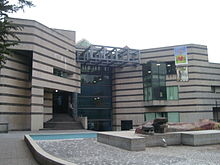
\includegraphics[scale=1]{IMG/26.jpg}
\caption{Facultad de Ciencias, UNAM.}
\label{fig:26}
\end{figure}

\chapter{Miguel Ángel Ordóñez}

\section{Yo}
Mi nombre es Miguel Ángel Ordóñez Silis. Nací el 5 de agosto de 1994 en la Ciudad de México.

\subsection{Hobbies}

Estos son algunos de los hobbies que tengo: 

\begin{itemize}
\item Videojuegos
\item Preparar café
\item Leer
\item Andar en bicicleta
\end{itemize}

\begin{figure}[h]
  \centering
  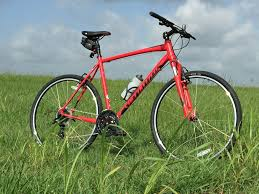
\includegraphics[scale=.5]{IMG27/27.jpg}
  \caption{Specialized Crosstrail Mech}
  \label{fig:bicicleta}
\end{figure}

\subsection{Libros}

Actualmente estoy leyendo \emph{Las cinco ecuaciones que cambiaron al mundo.~\cite{comunidad}}

\include{capitulo28}
\include{capitulo29}

\chapter{Bruno Martinez Enriquez}

Plantilla de \large{\LaTeX}
\section{Un poco sobre mí}

Soy Bruno, tengo 18 años, nací en la CDMX (cuando aún era DF) y he vivido aquí toda la vida.
Vengo de la ENP No. 7

Estoy citando este libro xd ~\cite{Floodlight}.

\subsection{hobbies}
\begin{itemize}
\item Jugar fútbol.
\item Jugar videojuegos
\item Ver televisión.
\end {itemize}

Tengo un pug que se llama Nacho
\begin{figure}[h]
  \centering
  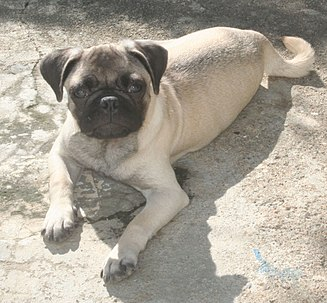
\includegraphics[scale=0.5]{IMG/30.jpg}
  \caption{No es él pero se parece.}
  \label{fig:pug}
\end{figure}

\include{capitulo31}




\bibliographystyle{acm}
\bibliography{bibliografia}
\end{document}

